\documentclass[border=2]{standalone}
\usepackage{tikz}
\usetikzlibrary{arrows, arrows.meta}

\begin{document}
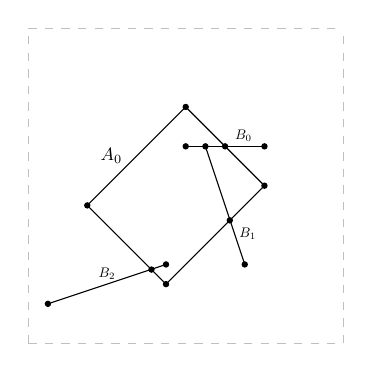
\begin{tikzpicture}
    \tikzstyle{node1}=[draw,scale=0.2,shape=circle,color=black,fill=black]
    
    \draw[color=black!25, style=dashed, step=4] (0,0) grid (4,4);

    \node[node1] (M) at (2,3) {};
    \node[node1] (R) at (3,2) {};
    \node[node1] (B)  at (0.75,1.75) {};
    \node[node1] (D)  at (1.75,0.75) {};
    
    \draw[] (B) -- node[midway, left = 1mm, scale=0.65]{$A_0$} (M);
    \draw[] (B) -- (D);
    \draw[] (D) -- (R); 
    \draw[] (M) -- (R);
    
    \node[node1] (B1) at (2.00, 2.50) {};
    \node[node1] (B2) at (2.25, 2.50) {};
    \node[node1] (B3) at (3.00, 2.50) {};
    \node[node1] (B4) at (2.75, 1.00) {};
    \draw[] (B1) -- node[pos=0.75, above = 0mm, scale = 0.5]{$B_0$} (B3);
    \draw[] (B2) -- node[pos=0.75, right = 0mm, scale = 0.5]{$B_1$} (B4);
    
    \node[node1] (B5) at (0.25, 0.50) {};
    \node[node1] (B6) at (1.75, 1.00) {};
    \draw[] (B5) -- node[midway, above = 0mm, scale = 0.5]{$B_2$} (B6);
    
    \node[node1] (I1) at (2.5,2.5) {};
    \node[node1] (I2) at (2.56,1.56) {};
    \node[node1] (I3) at (1.565,0.935) {};

\end{tikzpicture}
\end{document}
